\documentclass{article}
\usepackage[utf8]{inputenc}
\usepackage{amsmath}
\usepackage{amsfonts}
\usepackage{amssymb}
\usepackage{graphicx}
\usepackage{geometry}
\usepackage{xcolor}
\usepackage{gensymb}
\usepackage{hyperref}
\usepackage{gensymb}
\usepackage{listings}

\newcommand{\inv}{^{-1}}   
\newcommand{\Z}{\mathbb Z}
\newcommand{\R}{\mathbb R}
\newcommand{\Q}{\mathbb Q}
\newcommand{\C}{\mathbb C}
\newcommand{\N}{\mathbb N}

\begin{document}
\pagecolor{black}
\color{white}

\noindent{\bf 1.}
Let current flow to the right through the horizontal resistors, and down through the vertical resistors.
Then, $$I_1 = I_2 + I_3, ~~~ I_3 = I_4 + I_5,$$
and $$I_{1} = \frac{12-V_{a}}{1000}, ~~~ I_{2} = \frac{V_{a}-4}{2000}, ~~~ I_{3} = \frac{V_{a}-V_{b}}{10000}, ~~~ I_{4} = \frac{V_{b}}{1000}, ~~~ I_{5} = \frac{V_{b}}{3000}.$$
Then,
\begin{align*}
    I_{1}&=I_{2}+I_{3} \\
    \implies \frac{12-V_{a}}{1000}&=\frac{V_{a}-4}{2000}+\frac{V_{a}-V_{b}}{10000}, \\
    \implies V_a &= \frac{35}4 + \frac{1}{16}V_b.
\end{align*}
Thus,
\begin{align*}
    I_3 &= I_4 + I_5, \\
    \implies \frac{V_{a}-V_{b}}{10000}&=\frac{V_{b}}{1000}+\frac{V_{b}}{3000}, \\
    \implies V_{a}&=\frac{43}{3}V_{b}.
\end{align*}
Therefore,
\begin{align*}
    \frac{35}4 + \frac{1}{16}V_b &= \frac{43}{3}V_{b} \\
    \implies V_b &= \frac{29455}{144} \\
    &\approx 613.1\text{mV}.
\end{align*}

Now, we can solve for $V_a$:
\begin{align*}
    V_a &= \frac{43}3V_b \\
        &= \frac{1266565}{432} \\
        &\approx 8.788V
\end{align*}

Thus, $$I_{1} \approx 3.21\text{mA}, ~~~ I_{2} \approx 2.39\text{mA}, ~~~ I_{3} \approx 0.818\text{mA}, ~~~ I_{4} \approx 0.613\text{mA}, ~~~ I_{5} \approx 0.204\text{mA}.$$

\newpage\noindent{\bf 2.}

\begin{align*}
    \frac{V_{out}}{V_{in}} &= \frac{1}{\sqrt{1+(\omega RC)^2}}, \\
    \implies \frac{V_{out}}{\sin\left(1000t\right)} &= \frac{1}{\sqrt{1+\left(2\pi\cdot1000\cdot10000\cdot.2\cdot10^{-6}\right)^{2}}}, \\
    \implies V_{out} &= \frac{\sin\left(1000t\right)}{\sqrt{1+\left(2\pi\cdot1000\cdot10000\cdot.2\cdot10^{-6}\right)^{2}}} \\
            &= \frac{\sin\left(1000t\right)}{\sqrt{1+16\pi^{2}}}.
\end{align*}
Thus, the amplitude of the output wave is $\frac{1}{\sqrt{1+16\pi^{2}}} = 79.3$mV.

\begin{align*}
    \tan\phi &= \omega RC \\
             &= 2\pi\cdot1000\cdot10000\cdot.2\cdot10^{-6}, \\
    \implies \phi &= \arctan(4\pi) \\
                  &\approx 1.49.
\end{align*}
Thus, the phase shift of the output wave is 85.37\degree.

\newpage\noindent{\bf 3.}

The cut-off frequency is given by $$\omega_0 = \frac RL = \frac{50}{100\cdot10^{-6}} = \frac{50}{100\cdot10^{-6}} = 500000 \frac{\text{rad}}{\text{s}}$$
Thus, $$f = \frac{500000}{2\pi} \approx 79577\text{Hz}.$$

\newpage\noindent{\bf 4.}

At 0.4V amplitude, no current will flow in the diodes, so the circuit will be open and there will be no voltage drop across the resistor. Thus, the 0.4V sine wave is unchanged.
\begin{center}
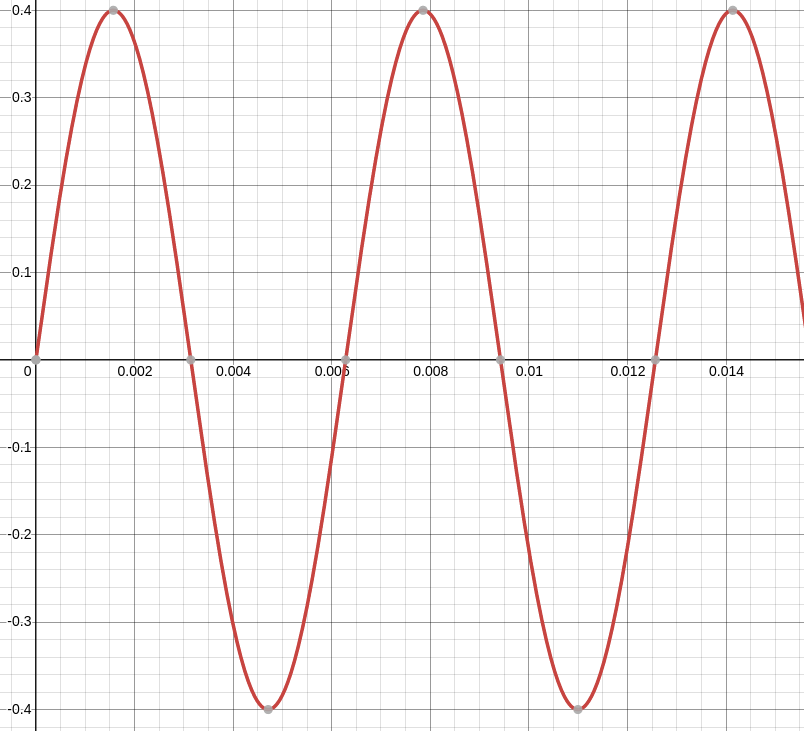
\includegraphics[scale=.3]{plot1.png}
\end{center}

At 0.7V amplitude, the diodes are activated for the portions of the wave above 0.6V and below -0.6V, so the peaks of the wave are flattened.
\begin{center}
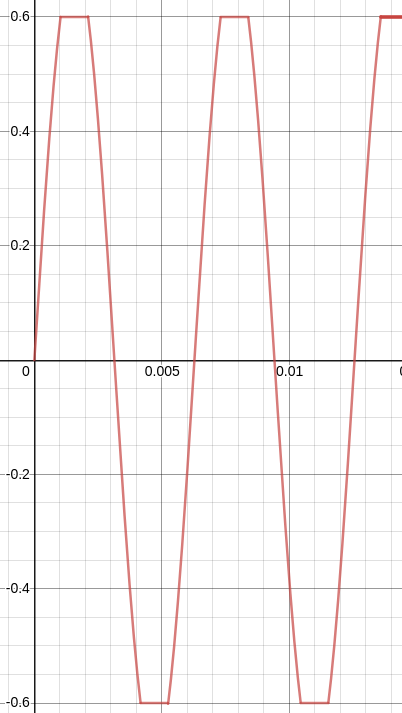
\includegraphics[scale=.5]{plot2.png}
\end{center}

\newpage
At 1V amplitude, the same logic applies.
\begin{center}
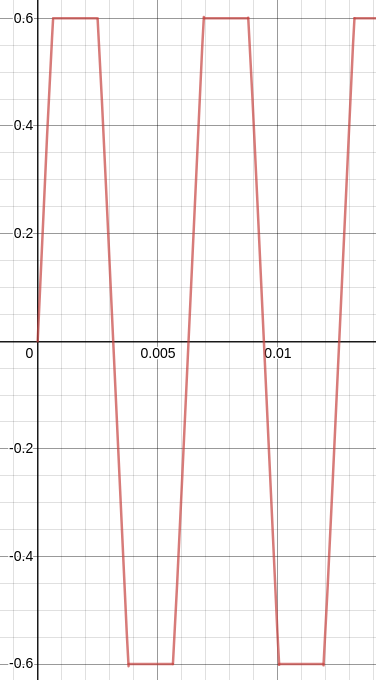
\includegraphics[scale=.5]{plot3.png}
\end{center}

\newpage\noindent{\bf 5.}

If the diode weren't in the circuit, the current in the circuit would be 60mA.
If the current were 60mA, then the voltage drop across the diode would be about 0.57V, according to the graph.
If that were the case, then the current in the circuit would be 54.3mA.
If the current were 54.3mA, then the voltage drop across the diode would be about 0.565V, according to the chart.
Iterating this process will give better and better approximations for the voltage at point $a$, but I don't think it will deviate too far from about 0.565V.

\newpage\noindent{\bf 6.}

    $$V_{\text{RMS}} = \sqrt2 \cdot 15 \approx 21.2V.$$

\newpage\noindent{\bf 7.}

    {\bf (a)} You need smaller filter capacitors for a bridge rectifier than you do for a half-wave rectifier because a full bridge rectifier's output frequency is twice its input frequency, so the capacitor needs to store less charge to provide current between peaks.

    {\bf (b)} A bridge rectifier and a full wave rectifier rated for the same voltage will have the same output, so they'll have the same capacitor requirements.

\newpage\noindent{\bf 8.}

    When $a$ is at its peak of 42.43V, $b$ is at 0V.
    Since D1 will cause a voltage drop of 0.6V, the peak output current will be $\frac{41.83}{3400} = 12.30$mA.
    Therefore, $$V_{\text{ripple}} = \frac{.01230}{120 \cdot .001} \approx 102.5\text{mV},$$
    $$V_{\text{out}} = \sqrt{2} \cdot 30 - 1.2 = 41.23\text{V}.$$


\newpage\noindent{\bf 9.}

\lstinputlisting[language=Python]{04.py}

\newpage\noindent{\bf 10.}

{\bf (a)}
Since no current will flow through the 2k resistor, the open circuit is equivalent to the following circuit:
\begin{center}
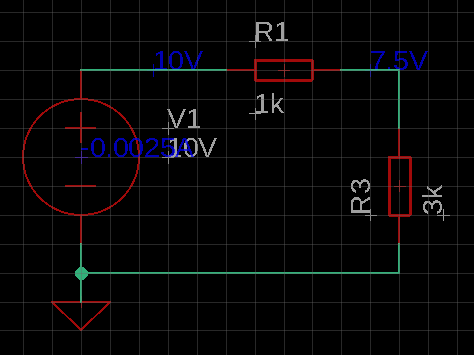
\includegraphics[scale=.5]{schematic04.png}
\end{center}
Thus, the open circuit voltage is 7.5V.

\medskip{\bf (b)}
\begin{center}
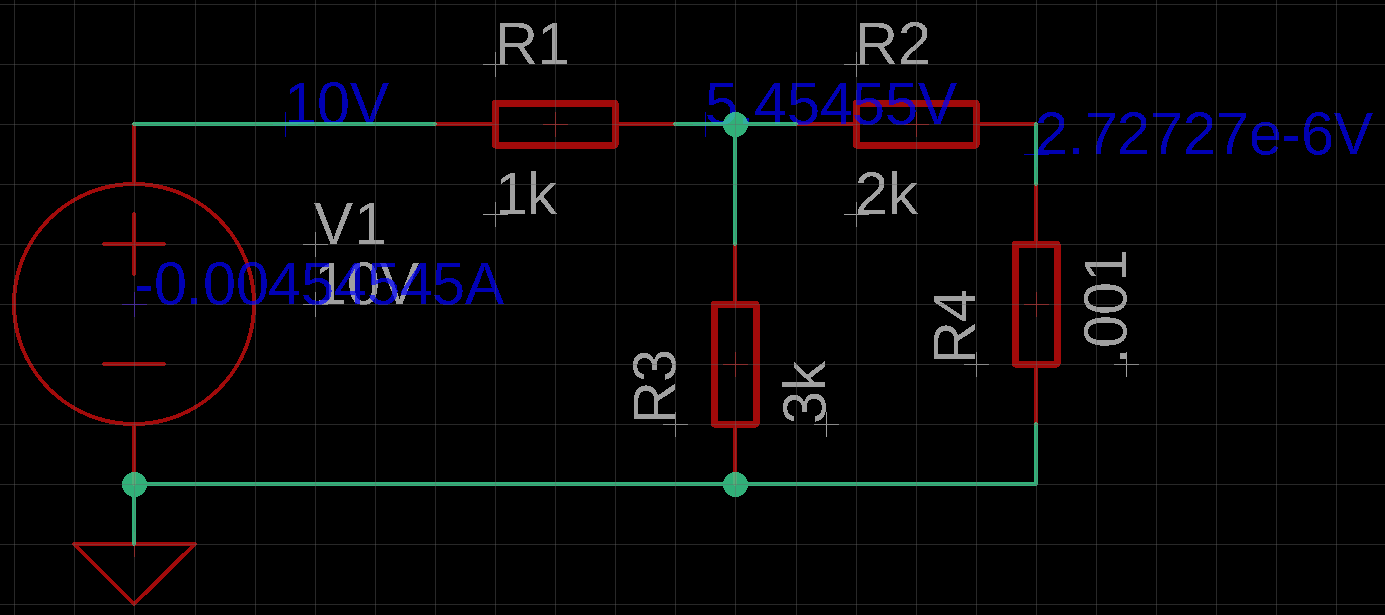
\includegraphics[scale=0.25]{schematic042.png}
\end{center}
Thus, the short circuit current is $$\frac{2.73 \cdot 10^{-6}}{.001} = 0.00273\text{A}.$$

\medskip{\bf (c)}
Thus, the Thévenin equivalent of the circuit consists of a 7.5V voltage source connected to a $\frac{7.5}{.00273} \approx 2747\Omega$ resistor.

\end{document}
